\documentclass[12pt, twoside]{article}
\usepackage[letterpaper, margin=1in, headsep=0.2in]{geometry}
\setlength{\headheight}{0.6in}
%\usepackage[english]{babel}
\usepackage[utf8]{inputenc}
\usepackage{microtype}
\usepackage{amsmath}
\usepackage{amssymb}
%\usepackage{amsfonts}
\usepackage{siunitx} %units in math. eg 20\milli\meter
\usepackage{yhmath} % for arcs, overparenth command
\usepackage{tikz} %graphics
\usetikzlibrary{quotes, angles}
\usepackage{graphicx} %consider setting \graphicspath{{images/}}
\usepackage{parskip} %no paragraph indent
\usepackage{enumitem}
\usepackage{multicol}
\usepackage{venndiagram}

\usepackage{fancyhdr}
\pagestyle{fancy}
\fancyhf{}
\renewcommand{\headrulewidth}{0pt} % disable the underline of the header
\raggedbottom
\hfuzz=2mm %suppresses overfull box warnings

\usepackage{hyperref}

\fancyhead[LE]{\thepage}
\fancyhead[RO]{\thepage \\ Name: \hspace{4cm} \,\\}
\fancyhead[LO]{BECA / Dr. Huson / Geometry\\*  Unit 8: Congruence transformations\\* 7 January 2023}

\begin{document}

\subsubsection*{8.5 Homework: Mixed congruence transformations \hfill CCSS.HSG.CO.A.5}
\begin{enumerate}
\item A translation maps triangle $DEF$ onto triangle $LMN$. \\[0.5cm]
  Write the letter or letters for each corresponding object. \vspace{0.5cm}
  \begin{multicols}{2}
    \begin{tikzpicture}[scale=1]
      \coordinate [label=above left:$L$](A) at (85:2);
      \coordinate [label=below:$M$](B) at (0, 0);
      \coordinate [label=right:$N$](C) at (25:3.5);
      \draw [thick] (A)--(B)--(C)--cycle;
      \draw [thick, xshift=-2cm, yshift=-3cm] (85:2) node[left]{$D$}--
      (0,0) node[below]{$E$}--
      (25:3.5) node[right]{$F$}--cycle;
    \end{tikzpicture}

    \begin{enumerate}
      \item $E \rightarrow$ \vspace{1.5cm}
      \item $F \rightarrow$ \vspace{1.5cm}
      \item $DF \rightarrow$ \vspace{1.5cm}
    \end{enumerate}
  \end{multicols}
  \begin{flushright}
    Auto scoring is turned on. Correct your errors.
  \end{flushright}
  
\item A translation maps $A$ to $A'$, as shown, $A(7,1) \rightarrow A'(2,3)$.
\begin{multicols}{2}
  \begin{enumerate}
    \item Which direction is the slide?
    \begin{enumerate}[label=(\Alph*)]
      \item Up, to the right
      \item Up, to the left
      \item Down, to the right
      \item Down, to the left
      \item None of the above
    \end{enumerate} \vspace{2cm}
    %\item What is the horizontal shift, how many squares right or left? \vspace{1.25cm}
    %\item What is the vertical shift, how many squares up or down? \vspace{1.25cm}
    \item If the same translation is applied to $C(6,3)\rightarrow C'(x,y)$, write the point $C'$ as an ordered pair in the box. (with parenthesis)
    \end{enumerate}
    \begin{flushright}
    \begin{tikzpicture}[scale=0.7]
      \draw [help lines] (-1,-2) grid (8,6);
      \draw [thick, ->] (-1.2,0) -- (8.4,0) node [below right] {$x$};
      \draw [thick, ->] (0,-2.2)--(0,6.4) node [left] {$y$};
      \draw [fill] (7,1) circle [radius=0.05] node[below] {$A(7,1)$};
      \draw [fill] (2,3) circle [radius=0.05] node[above] {$A'(2,3)$};
      \draw [->, dashed] (7,1)--(2,3);
      \draw [fill] (6,3) circle [radius=0.05] node[below] {$C(6,3)$};
    \end{tikzpicture}
    \end{flushright}
  \end{multicols}
  
\item Take notes: \emph{Reflection} is a transformation, also called ``flipping.'' Reflection is like looking in the mirror.
  \begin{enumerate}
    \item Lengths and angles are maintained (it is a rigid motion, or isometry)
    \item The \emph{orientation} is reversed. (letters are all backwards)
    \item The \emph{line of reflection} is a perpendicular bisector of the segment connecting a reflected point to its image.
  \end{enumerate}
  \begin{flushright}
    \begin{tikzpicture}[scale=1.0, rotate=30]
    \draw [thick, <->] (0,0) -- (8,0) node [above] {line of reflection};
    \draw [dashed, ->] (4,3)--(4,-2.9);
      \draw [fill] (4,3) circle [radius=0.05] node[above] {$P$};
      \draw [fill] (4,-3) circle [radius=0.05] node[below] {$P'$};
  \end{tikzpicture}
  \end{flushright}
  
\item Reflect the triangle across the $y$-axis, $\triangle ABC \rightarrow \triangle A'B'C'$. Complete the table of the coordinates and plot and label the image on the grid. \vspace{0.5cm}
\begin{multicols}{2}
  $A(1,2) \rightarrow$ \\[0.7cm]
  $B(1,4) \rightarrow$ \\[0.7cm]
  $C(4,2) \rightarrow$ \\[0.7cm]
    \begin{tikzpicture}[scale=.75]
    \draw [help lines] (-5,-2) grid (5,6);
    \draw [thick, <->] (-5.4,0) -- (5.4,0) node [right] {$x$};
    \draw [thick, <->] (0,-2.4)--(0,6.4) node [above] {$y$};  
    \draw [thick]
      (1,2) node[below left] {$A$}--
      (1,4) node[above left] {$B$}--
      (4,2) node[below] {$C$}--cycle;  
    \end{tikzpicture}
  \end{multicols}

\item $\triangle ABC$ is shown with vertices $A(-1,2)$, $B(6,1)$, and $C(5,4)$. Reflect the triangle across the $x$-axis. Write down its coordinates in a table and plot and label it on the graph.
  \begin{flushright}
    \begin{tikzpicture}[scale=0.7]
      \draw [help lines] (-3,-8) grid (8,8);
      \draw [thick, <->] (-3.4,0) -- (8.4,0) node [below right] {$x$};
      \draw [thick, <->] (0,-8.4)--(0,8.4) node [left] {$y$};
      \draw [thick] (-1,2) node[left] {$A$}--
        (6,1) node[right] {$B$}--
        (5,4) node[above right] {$C$}--
        cycle;
    \end{tikzpicture}
    \end{flushright}

\item The perimeter of the isosceles $\triangle FGH$ is $19 \frac{1}{2}$ with $\overline{FH} \cong \overline{GH}$. If $FG=x+2$ and $FH=8 \frac{1}{4}$, find $x$.\\[0.25cm]
    Show your work with an equation.\\[0.5cm]
      \begin{tikzpicture}[scale=0.5]
        \draw [thick](0,0)--(4,0)--(2,6)--(0,0);
        \draw [fill] (0,0) circle [radius=0.05] node[below left]{$F$};
        \draw [fill] (4,0) circle [radius=0.05] node[below right]{$G$};
        \draw [fill] (2,6) circle [radius=0.05] node[above right]{$H$};
        \draw [thick] (0.8,3.1)--(1.2,3); %tick mark
        \draw [thick] (2.8,3)--(3.2,3.1); %tick mark
        \node at (2,0) [below]{$x+2$};
        \node at (0.8,3.4) [left]{$8 \frac{1}{4}$};
      \end{tikzpicture}
      \begin{flushright}
        Write the value of $x$ in the box.
      \end{flushright}

\item A rotation maps triangle $DEF$ onto triangle $LMN$. \\[0.5cm]
Write the letter or letters for each corresponding object. \vspace{0.5cm}
    \begin{multicols}{2}
      \begin{tikzpicture}[scale=1]
        \coordinate [label=above left:$L$](A) at (85:2);
        \coordinate [label=above left:$M$](B) at (0, 0);
        \coordinate [label=right:$N$](C) at (25:3.5);
        \draw [thick] (A)--(B)--(C)--cycle;
        \draw [thick, rotate=-90] (85:2) node[right]{$D$}--
        (0,0) node[below left]{$E$}--
        (25:3.5) node[right]{$F$}--cycle;
      \end{tikzpicture}

      \begin{enumerate}
        \item $E \rightarrow$ \vspace{1.5cm}
        \item $F \rightarrow$ \vspace{1.5cm}
        \item $DF \rightarrow$ \vspace{1.5cm}
      \end{enumerate}
    \end{multicols}

\item A rotation centered at the origin maps $A$ to $A'$, as shown, $A(3,1) \rightarrow A'(-1,3)$.
\begin{multicols}{2}
  \begin{enumerate}
    \item Which correctly identifies the rotation?
    \begin{enumerate}[label=(\Alph*)]
      \item Clockwise $180^\circ$
      \item Counter clockwise $180^\circ$
      \item Clockwise $90^\circ$
      \item Counter clockwise $90^\circ$
      \item None of the above
    \end{enumerate} \vspace{2cm}
    %\item What is the horizontal shift, how many squares right or left? \vspace{1.25cm}
    %\item What is the vertical shift, how many squares up or down? \vspace{1.25cm}
    \item If the same translation is applied to $C(5,1)\rightarrow C'(x,y)$, plot and label the point $C'$ as an ordered pair.
    \end{enumerate}
    \begin{flushright}
    \begin{tikzpicture}[scale=0.7]
      \draw [help lines] (-3,-2) grid (8,6);
      \draw [thick, ->] (-3.2,0) -- (8.4,0) node [below right] {$x$};
      \draw [thick, ->] (0,-2.2)--(0,6.4) node [left] {$y$};
      \draw [fill] (3,1) circle [radius=0.05] node[below] {$A(3,1)$};
      \draw [fill] (-1,3) circle [radius=0.05] node[below left] {$A'(-1,3)$};
      %\draw [->, dashed] (7,1)--(2,3);
      \draw [fill] (5,1) circle [radius=0.05] node[right] {$C(5,1)$};
    \end{tikzpicture}
    \end{flushright}
\end{multicols}

\item Rotate the triangle $90^\circ$ clockwise around the origin, $\triangle ABC \rightarrow \triangle A'B'C'$. Complete the table of the coordinates and plot and label the image on the grid. \vspace{0.5cm}
\begin{multicols}{2}
  $A(1,2) \rightarrow$ \\[0.7cm]
  $B(1,4) \rightarrow$ \\[0.7cm]
  $C(4,2) \rightarrow$ \\[0.7cm]
    \begin{tikzpicture}[scale=.75]
    \draw [help lines] (-5,-5) grid (5,5);
    \draw [thick, <->] (-5.4,0) -- (5.4,0) node [right] {$x$};
    \draw [thick, <->] (0,-5.4)--(0,5.4) node [above] {$y$};  
    \draw [thick]
      (1,2) node[below left] {$A$}--
      (1,4) node[above left] {$B$}--
      (4,2) node[below] {$C$}--cycle;  
    \end{tikzpicture}
  \end{multicols}

\item $\triangle ABC$ is shown with vertices $A(-1,2)$, $B(6,1)$, and $C(5,4)$. Rotate the triangle $90^\circ$ counter clockwise around the origin. Write down its coordinates in a table and plot and label it on the graph.
  \begin{flushright}
    \begin{tikzpicture}[scale=0.7]
      \draw [help lines] (-7,-7) grid (7,7);
      \draw [thick, <->] (-7.4,0) -- (7.4,0) node [below right] {$x$};
      \draw [thick, <->] (0,-7.4)--(0,7.4) node [left] {$y$};
      \draw [thick] (-1,2) node[below] {$A$}--
        (6,1) node[right] {$B$}--
        (5,4) node[above right] {$C$}--
        cycle;
    \end{tikzpicture}
    \end{flushright}

\item The perimeter of the isosceles $\triangle FGH$ is $19 \frac{1}{2}$ with $\overline{FH} \cong \overline{GH}$. If $FG=x+2$ and $FH=8 \frac{1}{4}$, find $x$.\\[0.25cm]
    Show your work with an equation.\\[0.5cm]
      \begin{tikzpicture}[scale=0.5]
        \draw [thick](0,0)--(4,0)--(2,6)--(0,0);
        \draw [fill] (0,0) circle [radius=0.05] node[below left]{$F$};
        \draw [fill] (4,0) circle [radius=0.05] node[below right]{$G$};
        \draw [fill] (2,6) circle [radius=0.05] node[above right]{$H$};
        \draw [thick] (0.8,3.1)--(1.2,3); %tick mark
        \draw [thick] (2.8,3)--(3.2,3.1); %tick mark
        \node at (2,0) [below]{$x+2$};
        \node at (0.8,3.4) [left]{$8 \frac{1}{4}$};
      \end{tikzpicture}
      \begin{flushright}
        Write the value of $x$ in the box.
      \end{flushright}

\item A $110^\circ$ counterclockwise rotation centered at $P$ maps triangle $CAT$ onto triangle $DOG$. \\[0.5cm]
Write the letter or letters for each corresponding object. \vspace{0.5cm}
\begin{multicols}{2}
  \begin{tikzpicture}[scale=1.4, rotate=20]
    \coordinate [label=above left:$D$](A) at (65:2);
    \coordinate [label=below right:$O$](B) at (1, 0);
    \coordinate [label=right:$G$](C) at (15:3.5);
    \draw [thick] (A)--(B)--(C)--cycle;
    \draw [thick, rotate=-110] (65:2) node[right]{$C$}--
    (1,0) node[below left]{$A$}--
    (15:3.5) node[right]{$T$}--cycle;
    \draw [fill] (0,0) circle [radius=0.05] node[left] {$P$};
    \draw [dashed] (0,0) circle [radius=1];
  \end{tikzpicture}
  \begin{enumerate}
    \item $T \rightarrow$ \vspace{1.5cm}
    \item $A \rightarrow$ \vspace{1.5cm}
    \item $AC \rightarrow$ \vspace{1.5cm}
  \end{enumerate}
\end{multicols}

\item A translation maps $A$ to $A'$, as shown, $A(6,5) \rightarrow A'(2,2)$.
\begin{multicols}{2}
\begin{enumerate}
  \item Apply the same translation to $C(7,2)\rightarrow C'(x,y)$ on the grid. Mark and label point $C'$ as an ordered pair.
  \item Which direction is the slide?
  \begin{enumerate}[label=(\Alph*)]
    \item Up, to the right
    \item Up, to the left
    \item Down, to the right
    \item Down, to the left
    \item None of the above
  \end{enumerate} \vspace{2cm}
  \end{enumerate}
  \begin{flushright}
  \begin{tikzpicture}[scale=0.7]
    \draw [help lines] (-1,-4) grid (8,6);
    \draw [thick, ->] (-1.2,0) -- (8.4,0) node [below right] {$x$};
    \draw [thick, ->] (0,-4.2)--(0,6.4) node [left] {$y$};
    \draw [fill] (6,5) circle [radius=0.05] node[above] {$A(6,5)$};
    \draw [fill] (2,2) circle [radius=0.05] node[below] {$A'(2,2)$};
    \draw [->, dashed] (6,5)--(2.1,2.1);
    \draw [fill] (7,2) circle [radius=0.05] node[above] {$C(7,2)$};
  \end{tikzpicture}
  \end{flushright}
\end{multicols}

\item Complete the reflection diagram of $\triangle ABC \rightarrow \triangle A'B'C'$, below.
\begin{enumerate}
\item Label the triangle image.
\item True or false: reflection is a rigid motion.
\item Is the \emph{orientation} maintained or reversed by the reflection?
\item What is the degree measure of the angle between the \emph{line of reflection} and the dotted line segment from point $C$ to its image?
\end{enumerate}
\begin{flushright}
\begin{tikzpicture}[scale=0.8, rotate=40]
\draw [thick, <->] (0,0) -- (8,0) node [above] {line of reflection};
\draw [dashed, ->] (4,2)--(4,-1.9);
\draw [thick] (2,4)--(6,4)--(4,2)--cycle;
\draw [thick] (2,-4)--(6,-4)--(4,-2)--cycle;
  \draw [fill] (2,4) circle [radius=0.05] node[above left] {$A$};
  \draw [fill] (2,-4) circle [radius=0.05] node[below] {};
  \draw [fill] (6,4) circle [radius=0.05] node[above] {$B$};
  \draw [fill] (6,-4) circle [radius=0.05] node[below] {};
  \draw [fill] (4,2) circle [radius=0.05] node[below] {$C$};
  \draw [fill] (4,-2) circle [radius=0.05] node[below] {};
\end{tikzpicture}
\end{flushright}

\item A rotation centered at the origin maps $A$ to $A'$, as shown, $A(3,-1) \rightarrow A'(1,3)$.
\begin{multicols}{2}
\begin{enumerate}
  \item Apply the same rotation \\
  $C(5,1)\rightarrow C'(x,y)$, plotting and labeling the point $C'$ as an ordered pair.
  \item Which correctly identifies the rotation?
  \begin{enumerate}[label=(\Alph*)]
    \item Clockwise $180^\circ$
    \item Counter clockwise $180^\circ$
    \item Clockwise $90^\circ$
    \item Counter clockwise $90^\circ$
    \item None of the above
  \end{enumerate} \vspace{2cm}
  \end{enumerate}
  \begin{flushright}
  \begin{tikzpicture}[scale=0.7]
    \draw [help lines] (-3,-2) grid (8,6);
    \draw [thick, ->] (-3.2,0) -- (8.4,0) node [below right] {$x$};
    \draw [thick, ->] (0,-2.2)--(0,6.4) node [left] {$y$};
    \draw [fill] (3,-1) circle [radius=0.05] node[below] {$A(3,-1)$};
    \draw [fill] (1,3) circle [radius=0.05] node[below right] {$A'(1,3)$};
    %\draw [->, dashed] (7,1)--(2,3);
    \draw [fill] (5,1) circle [radius=0.05] node[right] {$C(5,1)$};
  \end{tikzpicture}
  \end{flushright}
\end{multicols}

\item Reflect the triangle across the $x$-axis, $\triangle ABC \rightarrow \triangle A'B'C'$. Complete the table of the coordinates and plot and label the image on the grid. \vspace{0.5cm}
\begin{multicols}{2}
$A(1,2) \rightarrow$ \\[0.7cm]
$B(1,4) \rightarrow$ \\[0.7cm]
$C(4,2) \rightarrow$ \\[0.7cm]
  \begin{tikzpicture}[scale=.75]
  \draw [help lines] (-5,-5) grid (5,5);
  \draw [thick, <->] (-5.4,0) -- (5.4,0) node [right] {$x$};
  \draw [thick, <->] (0,-5.4)--(0,5.4) node [above] {$y$};  
  \draw [thick]
    (1,2) node[below left] {$A$}--
    (1,4) node[above left] {$B$}--
    (4,2) node[below] {$C$}--cycle;  
  \end{tikzpicture}
\end{multicols}

\item $\triangle ABC$ is shown with vertices $A(-1,2)$, $B(4,1)$, and $C(6,4)$. Rotate the triangle $90^\circ$ clockwise around the origin. Write down its coordinates in a table and plot and label it on the graph.
\begin{flushright}
  \begin{tikzpicture}[scale=0.7]
    \draw [help lines] (-7,-7) grid (7,7);
    \draw [thick, <->] (-7.4,0) -- (7.4,0) node [below right] {$x$};
    \draw [thick, <->] (0,-7.4)--(0,7.4) node [left] {$y$};
    \draw [thick] (-1,2) node[below] {$A$}--
      (4,1) node[right] {$B$}--
      (6,4) node[above right] {$C$}--
      cycle;
  \end{tikzpicture}
  \end{flushright}

\item A composition of two transformations is applied to $\triangle ABC$, shown in the diagram. Fully characterize the two transformations, in order.
  \begin{flushright}
    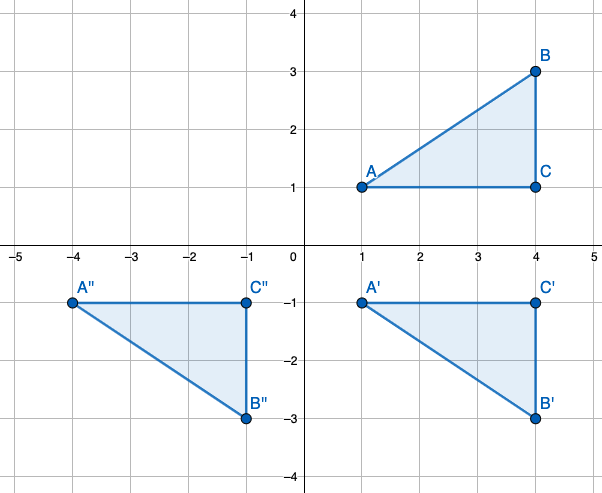
\includegraphics[width=5in]{../graphics/08reflect+translate.png}
  \end{flushright}

\item A point labeled $A$ and vector $(-3,1)$ are shown Geogebra/classic. Identify the following objects and tools.
\begin{enumerate}
  \item Circle the vector
  \item Make an ``X'' where to click for the menu ``Name \& Value'' that will label point $A$ as an ordered pair.
  \item Mark with an arrow the menu where the ``Translate by vector'' tool is found.
\end{enumerate}
\begin{flushright}
  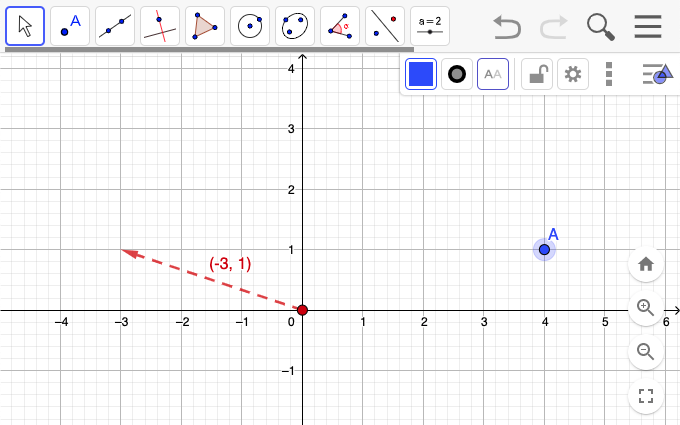
\includegraphics[width=6.25in]{../graphics/08Geogebra_toolbar.png}
\end{flushright}

\item Perform a composition of two transformations using Geogebra/classic. Paste an image of your work in this Classkick slide using the ``camera'' tool.
  \begin{enumerate}
    \item Plot $\triangle ABC$, $A(1,2)$, $B(4,3)$, $C(5,6)$
    \item Mark a point at the origin.
    \item Rotate the triangle $90^\circ$ clockwise around the origin.
    \item Reflect the image $\triangle A'B'C'$ across the $y$-axis.
  \end{enumerate}          

\item A reflection is performed on a triangle, $\triangle SIT \rightarrow \triangle RUN$, as shown below. \\[0.5cm]
Write the letter or letters for each corresponding object. \vspace{0.5cm}
  \begin{multicols}{2}
  \begin{tikzpicture}[scale=0.9, rotate=-40]
  \draw [thick, <->] (0,0) -- (7,0) node [below] {line of reflection};
  \draw [dashed, ->] (3.1,1.3)--(3.1,-1.3);
  \draw [thick] (2,3)--(6,3)--(3.1,1.3)--cycle;
  \draw [thick] (2,-3)--(6,-3)--(3.1,-1.3)--cycle;
  \draw [fill] (2,3) circle [radius=0.05] node[above left] {$S$};
  \draw [fill] (2,-3) circle [radius=0.05] node[above] {$R$};
  \draw [fill] (6,3) circle [radius=0.05] node[below] {$I$};
  \draw [fill] (6,-3) circle [radius=0.05] node[below] {$U$};
  \draw [fill] (3.1,1.3) circle [radius=0.05] node[above left] {$T$};
  \draw [fill] (3.1,-1.3) circle [radius=0.05] node[right] {$N$};
  \end{tikzpicture}
  \begin{enumerate}
  \item $S \rightarrow$ \vspace{1.5cm}
  \item $T \rightarrow$ \vspace{1.5cm}
  \item $SI \rightarrow$ \vspace{1.5cm}
  \end{enumerate}
  \end{multicols}


\item A translation maps $A$ to $A'$, as shown, $A(1,3) \rightarrow A'(4,-2)$.
\begin{multicols}{2}
  \begin{enumerate}
  \item Apply the same translation to $B(4,4)\rightarrow B'(x,y)$ on the grid. Mark and label point $B'$ as an ordered pair.
  \item Which translation mapped $A \rightarrow A'$?
  \begin{enumerate}[label=(\Alph*)]
    \item Right 3, up 1
    \item Left 3, down 1
    \item Right 5, down 3
    \item Right 3, down 5
    \item None of the above
  \end{enumerate} \vspace{2cm}
  \end{enumerate}
  \begin{flushright}
  \begin{tikzpicture}[scale=0.7]
    \draw [help lines] (-1,-4) grid (8,6);
    \draw [thick, ->] (-1.2,0) -- (8.4,0) node [below right] {$x$};
    \draw [thick, ->] (0,-4.2)--(0,6.4) node [left] {$y$};
    \draw [fill] (1,3) circle [radius=0.05] node[above] {$A(1,3)$};
    \draw [fill] (4, -2) circle [radius=0.05] node[below left] {$A'(4,-2)$};
    \draw [->, dashed] (1,3)--(3.9,-1.9);
    \draw [fill] (4,4) circle [radius=0.05] node[above] {$B(4,4)$};
  \end{tikzpicture}
  \end{flushright}
\end{multicols}

\item A $70^\circ$ clockwise rotation centered at $P$ maps $\triangle ABC \rightarrow \triangle A'B'C'$, below.
\begin{enumerate}
  \item Complete the diagram by labeling the vertices of the triangle image.\\(remember the primes)
  \item True or false: rotation is a rigid motion.
  \item Is the \emph{orientation} maintained or reversed by the rotation?
\end{enumerate}
\begin{flushright}
  \begin{tikzpicture}[scale=1.4, rotate=-10]
    \coordinate [label=above right:$A$](A) at (55:1);
    \coordinate [label=below right:$B$](B) at (2, 0);
    \coordinate [label=right:$C$](C) at (15:3.5);
    \draw [thick] (A)--(B)--(C)--cycle;
    \draw [thick, rotate=-70] (55:1) node[right]{}--
    (2,0) node[below left]{}--
    (15:3.5) node[right]{}--cycle;
    \draw [fill] (0,0) circle [radius=0.05] node[left] {$P$};
    \draw [dashed] (0,0) circle [radius=1];
  \end{tikzpicture}
\end{flushright}

\item A reflection is performed on a line segment, mapping $\overline{AB} \rightarrow \overline{A'B'}$, as shown.
\begin{multicols}{2}
  \begin{enumerate}
    \item Apply the same reflection to $C$. \\
    Plot and label the image $C'$ as an ordered pair.
    \item Which correctly identifies the reflection?
    \begin{enumerate}[label=(\Alph*)]
      \item Reflect over the $x$-axis
      \item Reflect over the $y$-axis
      \item Reflect over the $x$-axis, then the $y$-axis
      \item Reflect over the $y$-axis, then the $x$-axis
      \item None of the above
    \end{enumerate} \vspace{2cm}
    \end{enumerate}
    \begin{flushright}
    \begin{tikzpicture}[scale=0.7]
      \draw [help lines] (-5,-2) grid (6,6);
      \draw [thick, ->] (-5.2,0) -- (6.4,0) node [below right] {$x$};
      \draw [thick, ->] (0,-2.2)--(0,6.4) node [left] {$y$};
      \draw [thick] (2,5)--(2,3);
      \draw [fill] (2,5) circle [radius=0.05] node[above] {$A(2,5)$};
      \draw [fill] (2,3) circle [radius=0.05] node[below] {$B(2,3)$};
      \draw [thick] (-2,5)--(-2,3);
      \draw [fill] (-2,5) circle [radius=0.05] node[above] {$A'(-2,5)$};
      \draw [fill] (-2,3) circle [radius=0.05] node[below] {$B'(-2,3)$};
      %\draw [->, dashed] (7,1)--(2,3);
      \draw [fill] (4,1) circle [radius=0.05] node[below] {$C(4,1)$};
    \end{tikzpicture}
    \end{flushright}
\end{multicols}

\item What are the two transformations applied mapping $\triangle ABC \rightarrow \triangle A'B'C' \rightarrow \triangle A''B''C''$, as shown in the diagram? \emph{Fully characterize} the two transformations, in order.
    \begin{flushright}
      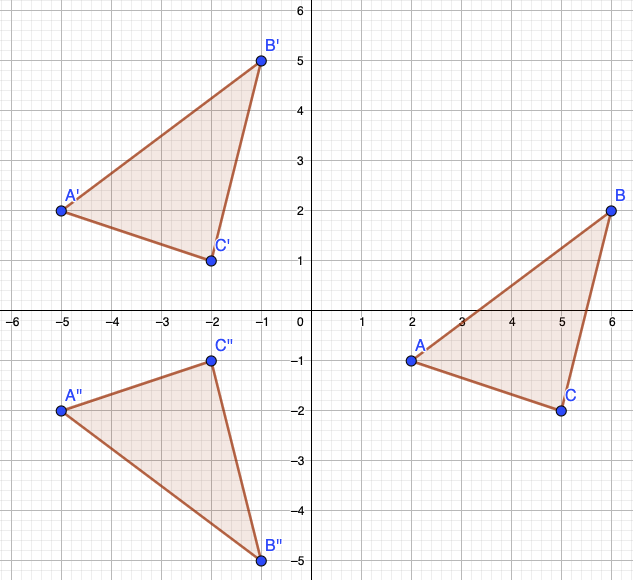
\includegraphics[width=6in]{../graphics/08Translate+reflect.png}
    \end{flushright}

\item Rotate the triangle $180^\circ$ counterclockwise around the origin, $\triangle ABC \rightarrow \triangle A'B'C'$. Complete the table of the coordinates and plot and label the image on the grid. \vspace{0.5cm}
\begin{multicols}{2}
  $A(0,0) \rightarrow$ \\[0.7cm]
  $B(4,2) \rightarrow$ \\[0.7cm]
  $C(4,0) \rightarrow$ \\[0.7cm]
    \begin{tikzpicture}[scale=.75]
    \draw [help lines] (-5,-5) grid (5,5);
    \draw [thick, <->] (-5.4,0) -- (5.4,0) node [right] {$x$};
    \draw [thick, <->] (0,-5.4)--(0,5.4) node [above] {$y$};  
    \draw [thick]
      (0,0) node[below right] {$A$}--
      (4,2) node[above left] {$B$}--
      (4,0) node[below] {$C$}--cycle;  
    \end{tikzpicture}
  \end{multicols}
  
\item $\triangle ABC$ is shown with vertices $A(1,2)$, $B(5,1)$, and $C(6,4)$. First, translate the triangle left 7 and up 2, then reflect it across the $x$-axis. \\[0.5cm]
Plot and label $\triangle A'B'C'$ and $\triangle A''B''C''$ on the graph.
  \begin{center}
    \begin{tikzpicture}[scale=0.8]
      \draw [help lines] (-8,-8) grid (8,8);
      \draw [thick, <->] (-8.4,0) -- (8.4,0) node [below right] {$x$};
      \draw [thick, <->] (0,-8.4)--(0,8.4) node [left] {$y$};
      \draw [thick] (1,2) node[below] {$A$}--
        (5,1) node[right] {$B$}--
        (6,4) node[above right] {$C$}--
        cycle;
    \end{tikzpicture}
    \end{center}

\item A point labeled $C$ and vector $(1,3)$ are shown Geogebra/classic. Identify the following objects and tools.
  \begin{enumerate}
    \item Circle the vector
    \item Make an ``X'' where to click for the menu ``Name \& Value'' that will label point $C$ as an ordered pair.
    \item Mark with an arrow the menu where the ``Translate by vector'' tool is found.
  \end{enumerate}
  \begin{flushright}
    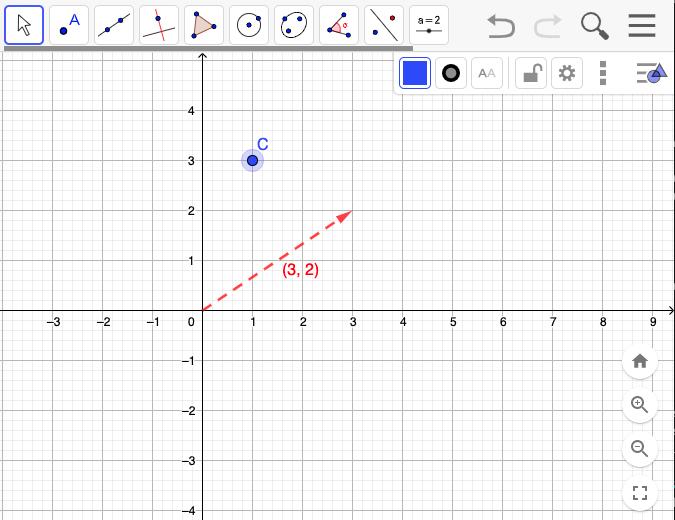
\includegraphics[width=6in]{../graphics/08bGeogebra_toolbar.png}
  \end{flushright}

\item Perform a composition of two transformations using Geogebra/classic. Paste an image of your work in this Classkick slide using the ``camera'' tool.
  \begin{enumerate}
    \item Plot $\triangle ABC$, $A(2,1)$, $B(5,4)$, $C(5,1)$
    \item Mark a point at the origin.
    \item Rotate the triangle $180^\circ$ counter clockwise around the origin.
    \item Reflect the image $\triangle A'B'C'$ across the $y$-axis, producing $\triangle A''B''C''$.
  \end{enumerate}

\newpage
\item Plot the parallelogram $BECA$ with $B(-2,-1)$, $E(3,-1)$, $C(2,-4)$, and $A(-3,-4)$. Translate the quadrilateral up 5 and right 2, labeling it $B'E'C'A'$. (use a straight edge for full credit)
    \begin{center}
      \begin{tikzpicture}[scale=0.9]
      \draw [help lines] (-5,-5) grid (5,5);
      \draw [thick, <->] (-5.4,0) -- (5.4,0) node [right] {$x$};
      \draw [thick, <->] (0,-5.4)--(0,5.4) node [above] {$y$};
      \foreach \x in {-5,...,-1,1,2,3,4,5}
        \draw[shift={(\x,0)},color=black] (0pt,-3pt) -- (0pt,3pt) node[below=5pt]  {$\x$};
      \foreach \y in {-5,...,-1,1,2,3,4,5}
        \draw[shift={(0,\y)},color=black] (-3pt,0pt) -- (3pt,0pt) node[left=5pt]  {$\y$}; 
    \end{tikzpicture}
  \end{center}
  
\item Reflect the triangle over the $x$-axis, $\triangle ABC \rightarrow \triangle A'B'C'$. Complete the table of the coordinates and plot and label the image on the grid. \vspace{0.5cm}
  \begin{multicols}{2}
    $A(1,2) \rightarrow$ \\[0.7cm]
    $B(1,4) \rightarrow$ \\[0.7cm]
    $C(4,2) \rightarrow$ \\[0.7cm]
      \begin{tikzpicture}[scale=.75]
      \draw [help lines] (-5,-5) grid (5,5);
      \draw [thick, <->] (-5.4,0) -- (5.4,0) node [right] {$x$};
      \draw [thick, <->] (0,-5.4)--(0,5.4) node [above] {$y$};  
      \draw [thick]
        (1,2) node[below left] {$A$}--
        (1,4) node[above left] {$B$}--
        (4,2) node[below] {$C$}--cycle;  
      \end{tikzpicture}
    \end{multicols}

\newpage
\item A translation is performed mapping $(x,y) \rightarrow (x+4, y-1)$.
\begin{multicols}{2}
  \begin{enumerate}
    \item What is the horizontal shift, how many squares right or left? \vspace{1cm}
    \item What is the vertical shift, how many squares up or down? \vspace{1cm}
    \item Identify the image of point $A$. $A(-1,2)\rightarrow$
  \end{enumerate}
    \begin{tikzpicture}[scale=0.7]
      \draw [help lines] (-3,-2) grid (8,6);
      \draw [thick, ->] (-3.2,0) -- (8.4,0) node [below right] {$x$};
      \draw [thick, ->] (0,-2.2)--(0,6.4) node [left] {$y$};
      \draw [fill] (3,1) circle [radius=0.05] node[below] {$B(3,1)$};
      \draw [fill] (-1,2) circle [radius=0.05] node[below left] {$A(-1,2)$};
      %\draw [->, dashed] (7,1)--(2,3);
      \draw [fill] (3,3) circle [radius=0.05] node[above] {$C(3,3)$};
    \end{tikzpicture}
  \end{multicols} \vspace{1cm}

\item In the diagram below, $\triangle ABC$ with sides of 13, 15, and 16, is mapped onto $\triangle DEF$ after a clockwise rotation of $90^\circ$ about point $P$. 
  \begin{multicols}{2}
    \begin{enumerate}
      \item What is $A$ mapped to? $A \rightarrow$ \vspace{1.5cm}
      \item What corresponds to $F$? \vspace{1.5cm}
      \item Given $DE=2x-1$. Find $x$. \vspace{1.5cm}
    \end{enumerate}
    \begin{tikzpicture}[scale=.6]
      %\draw [thick, <->] (-7.4,0) -- (10.4,0) node [right] {$x$};
      %draw [thick, <->] (0,-5.4)--(0,10.4) node [above] {$y$};
      \fill (0,0) circle[radius=0.1] node[right]{$P$};
      \draw [thick]
        (-2,1) node[below left] {$A$}--
        (-7,2) node[left] {$B$}--
        (-4,5) node[above right] {$C$}--cycle;
        \node at (-5,1.5)[below]{16};
        \node at (-6,4){13};
        \node at (-2.5,3.5){15};
        \node at (0.25,5){$2x-1$};
      \draw [thick]
        (1,2) node[left] {$D$}--
        (2,7) node[above] {$E$}--
        (5,4) node[right] {$F$}--cycle;
    \end{tikzpicture}
  \end{multicols}
  \vspace{3cm}

\item A translation maps $D(2,4) \rightarrow D'(-3,4)$. What is the image of $E(5,-5)$ under the same translation?

\newpage
\item The triangle $ABC$, shown below, undergoes two rigid motions carrying it onto triangle $XYZ$. State the two isometric transformations. (be specific)
  \begin{flushright}
    \begin{tikzpicture}[scale=.48]
      \draw [help lines] (-10,-6) grid (10,10);
      \draw [thick, <->] (-10.4,0) -- (10.4,0) node [right] {$x$};
      \draw [thick, <->] (0,-6.4)--(0,10.4) node [above] {$y$};
      \draw [thick]
        (4,2) node[below left] {$X$}--
        (8,3) node[right] {$Y$}--
        (8,6) node[above right] {$Z$}--cycle;
      \draw [thick]
        (-1,1) node[below left] {$A$}--
        (-2,5) node[above right] {$B$}--
        (-5,5) node[above left] {$C$}--cycle;
    \end{tikzpicture}
  \end{flushright}

\item Triangle $\triangle ABC$ is graphed on the set of axes below. The vertices of $\triangle ABC$ have the coordinates $A(2,-3)$, $B(8,1)$, and $C(-1,8)$. \\*[0.25cm]
Reflect the triangle across the $y$-axis. Write down its coordinates in a table and plot and label it on the graph.
    \begin{flushright} %4 quadrant regents grid
    \begin{tikzpicture}[scale=.48]
      \draw [help lines] (-9,-5) grid (10,9);
      \draw [thick, <->] (-9.4,0) -- (10.4,0) node [below right] {$x$};
      \draw [thick, <->] (0,-5.4)--(0,9.4) node [left] {$y$};
      \draw [thick] (2,-3) node[below] {$A$}--
      (8,1) node[right] {$B$}--
      (-1,8) node[left] {$C$}--
      cycle;
      %\draw [fill] (5,0) circle [radius=0.1] node[above left] {$P$};
    \end{tikzpicture}
    \end{flushright}



\end{enumerate}
\end{document}